\chapter{Implementazione: CNN}
\label{ch:CNN}
\section{Creazione rete neurale}
Lo sviluppo della rete neurale convoluzionale, per effettuare previsioni partendo dalle immagini, è basata sulla rete 
MobileNetV2. L'uso di tale rete come base consente di usare dei pesi preallenati in modo da rendere il processo di training sul dataset più efficiente.
\\\\
Tuttavia tale processo necessita di alcune fasi aggiuntive per fare in modo che la rete riesca a prendere i dati della dimensione esatta 
e restituire delle previsioni nell'insieme desiderato.
\\\\
Tali operazioni sono:
\begin{itemize}
    \item Inserire la dimensione delle immagini nel layer di input
    \item Effettuare fine tuning e transfer learning per poter usare i pesi preallenati 
    \item Inserire dei layer finali per ottenere degli output significativi
\end{itemize}

La dimensione scelta delle immagini è (224x224), dunque la rete prende in ingresso degli array di dimensione 224x224x3 (dove quest'ultimo indica l'uso dei colori RGB).
Per tale motivo il layer di input deve accettare tale dimensione.
\\\\
I pesi preallenati che si sono scelti sono pesi allenati su ImageNet. ImageNet è un dataset di immagini suddivise in 1000 classi. Il dataset su cui si deve svolgere il training, tuttavia, possiede 
unicamente una classe, per via del fatto che abbiamo trasformato il valore della prognosi da una string ad un valore binario. 
Per cui l'immagine può appartenere o meno a tale classe.
\\\\
Al fine di poter usare tali pesi per effettuare il training, si necessita dunque di ulteriori passaggi: 
\begin{itemize}
    \item Transfer Learning
    \item Fine tuning
\end{itemize}

\section{Transfer Learning}

Il transfer learning consente di sfruttare la rete già allenata a risolvere problemi diversi, ma comunque correlati con quello di interesse.
Nel caso considerato tale tecnica permette di usare una rete allenata per prevedere l'appartenenza di una immagine ad una delle 1000 classi di ImageNet
per creare una rete in grado di classificare le immagini del dataset in una unica classe.
\\\\
Per sfruttare la rete allenata, congeliamo lo stato dei layer di classificazione, al fine di non alterarli, e settiamo la rete come non allenabile.
In tal modo si è ottenuto un nuovo modello basato sulla MobileNetV2.
\\\\
Ora si presenta un problema relativo alla classificazione. Per ovviare al fatto che tale operazione sarà fatta per una sola classe, si necessita dell'inserimento di altri layer alla fine del modello precedentemente ottenuto.
\\\\
Tali layers sono:
\begin{itemize}
    \item un GlobalAveragePooling2D()
    \item due Dense() 
\end{itemize}  

Il primo layer serve per via del fatto che allo stato attuale la rete produce un output multidimensionale e, per ottenere previsioni formate da un singolo vettore 
della dimensione prevista, usiamo tale layer, il quale genera previsioni basate sul blocco multidimensionale e facendone una media.
\\\\
Il primo Dense layer viene usato per generare l'output prodotto dalle immagini dei polmoni. Tale layer è formato da 100 neuroni ed ha come funzione di attivazione ReLu.
\\\\
Il secondo Dense layer svolge il lavoro di classificazione vero e proprio. Per via del fatto che si è scelto di usare una label binaria, ovvero classifichiamo su un'unica classe, tale 
layer è composto da un solo neurone, ed ha come funzione di attivazione Sigmoid.
\\\\
Una volta creati i layers, per completare la fase di transfer learning, si deve compilare il modello finale, ottenuto aggiungendo i nuovi layers.
\\\\
Ora la rete è pronta per una prima fase di training. In tale fase sono stati usati i seguenti parametri per il training:
\begin{itemize}
    \item Loss function: Adam
    \item Metrica: accuracy
    \item Epoche 150
    \item Batch size: 30
\end{itemize}
$\\$
Per quanto concerne il valore del learning rate sono si è deciso di effettuare prove sia con $10^{-3}$ che con 
$10^{-4}$.
I risultati ottenuti dal training sono espressi nei seguenti grafici.

\begin{figure}[h]
    \centering
    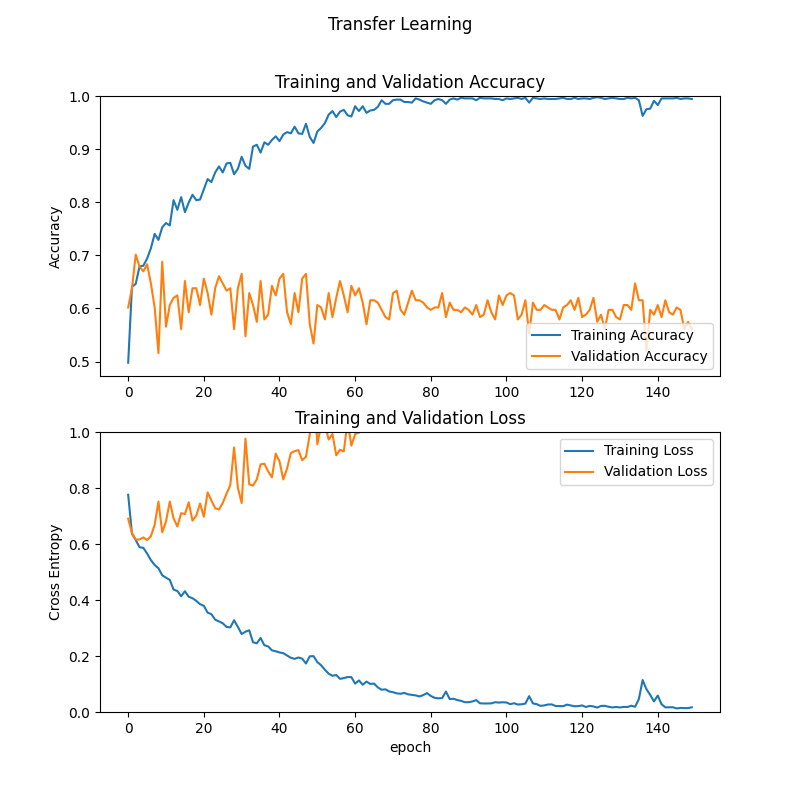
\includegraphics[width=12cm]{./10-3_150.png}
    \label{ 10^{-3} }
    \caption{Test effettuato usando come learning rate $10^{-3}$}
\end{figure}

\begin{figure}[ht]
    \centering
    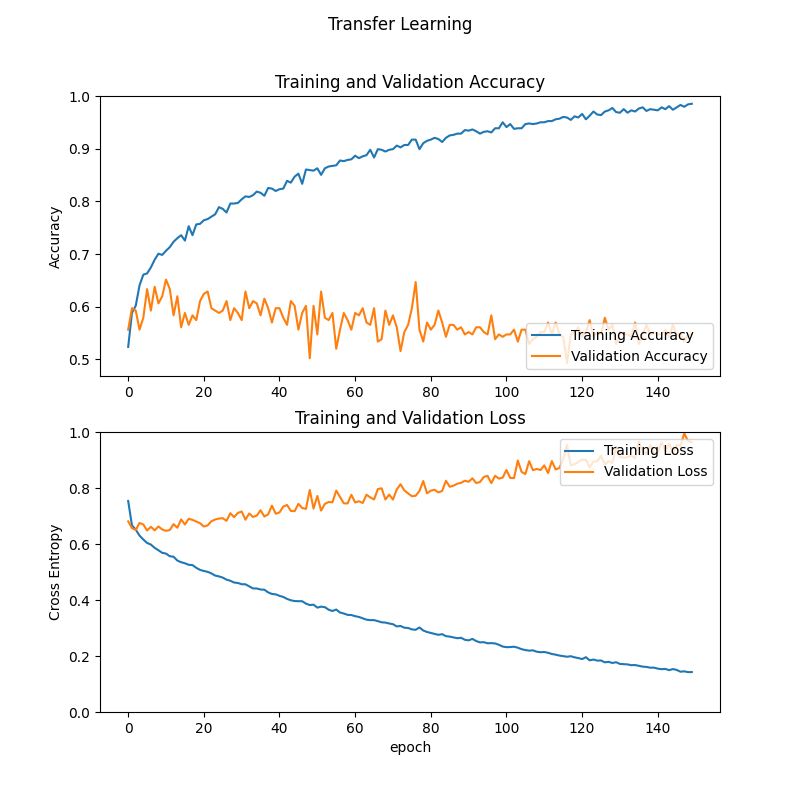
\includegraphics[width=12cm]{./10-4_150.png}
    \label{10^{-4}}
    \caption{Test effettuato usando come learning rate $10^{-4}$}
\end{figure}
\vspace{1000mm}

\section{Fine Tuning}

Per procedere con la fase di fine tuning, si deve rendere nuovamente trainabile il modello creato, 
in modo tale che i pesi possano essere allenati considerando i nuovi layers.
Così facendo si permette ai pesi di regolarsi sul dataset d'interesse, partendo da quello su cui sono stati inizialmente allenati.
\\\\
Essendo gli ultimi layers di una rete inutili in termini di classificazione, possiamo decidere di 
congelarli, ovvero non considerarli durante il training, in modo da risparmiare risorse.
Effettuato tale passaggio si può procedere con la compilazione del modello ottenuto e procedere con il training.
\\\\
I parametri relativi al training in questa fase sono:
\begin{itemize}
    \item Loss function: Adam
    \item Metrica: accuracy
    \item Epoche 30
    \item Batch size: 30
\end{itemize}
$\\$
Di seguito sono riportati i risultati ottenuti a seguito del transfer learning e fine tuning, sempre considerando 
i due valori scelti per il learning rate.

\begin{figure}[h]
    \centering
    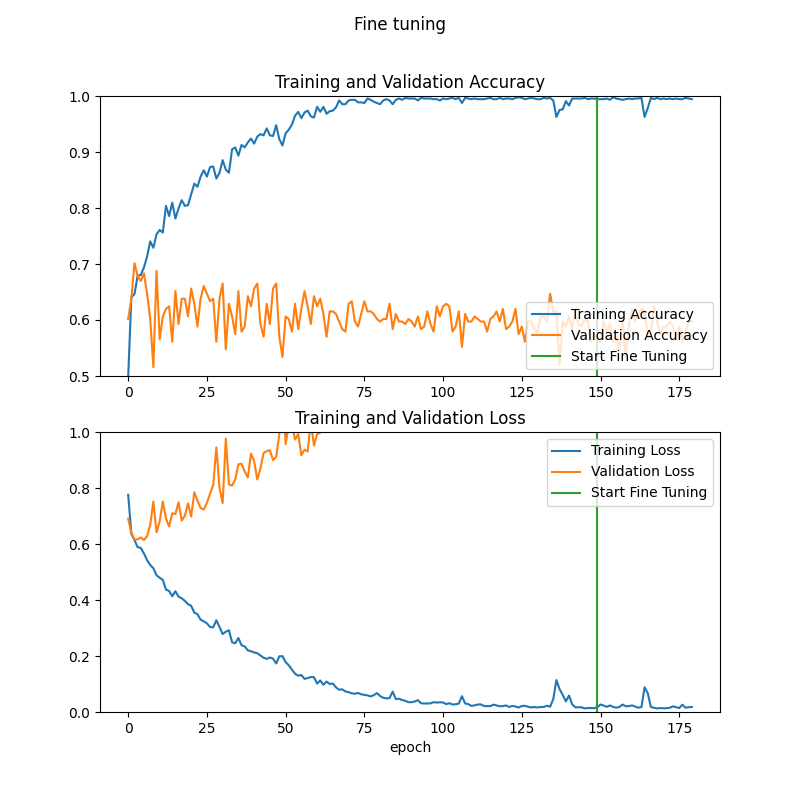
\includegraphics[width=12cm]{./10-3_150_2.png}
    \label{ 10^{-3} }
    \caption{Test effettuato usando come learning rate $10^{-3}$}
\end{figure}

\begin{figure}[t]
    \centering
    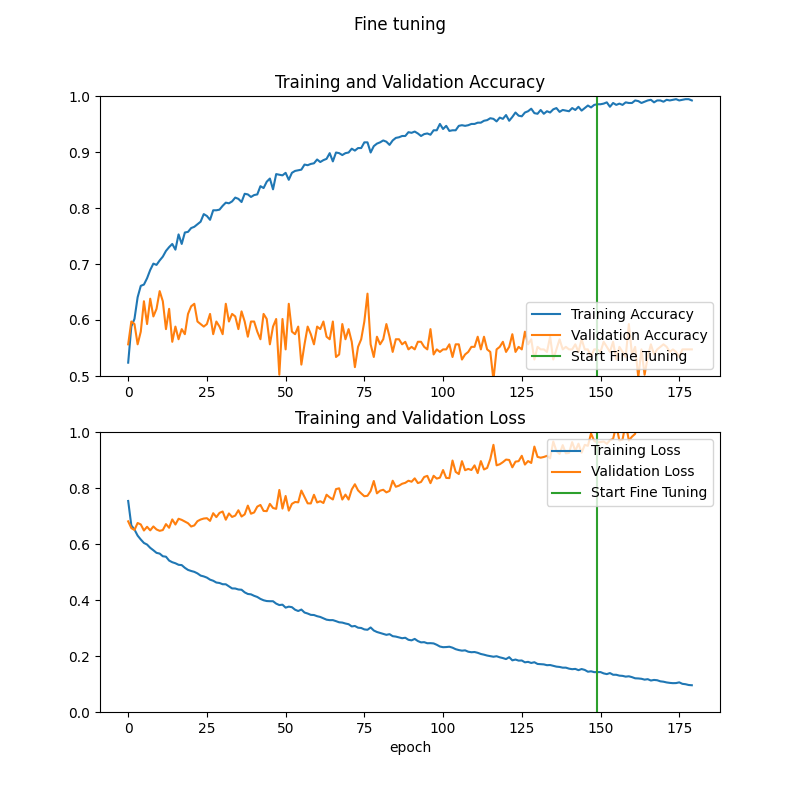
\includegraphics[width=12cm]{./10-4_150_2.png}
    \label{10^{-4}}
    \caption{Test effettuato usando come learning rate $10^{-4}$}
\end{figure}
\vspace{1000mm}
\section{Overfit e Data Augmentation}
Dai risultati ottenuti risulta evidente la presenza di overfitting nella rete.
Tale problema si è potuto notare per via del fatto che, anche a seguito del fine tuning, la validation accuracy non tende 
ad aumentare.
\\\\
L'overfit può essere causato dal fatto che la rete si abitui agli input del training set, o al 
fatto che questi siano molto simili tra di loro e risponda in maniera casuale a nuovi dati. Per tale motivo si è scelto di usare la data augmentation come tecnica risolutiva.
La data augmentation consiste nel prendere le immagini del dataset, effettuare delle modifiche ad esse (come rotazioni), per 
creare una immagine nuova, in modo da introdurre diversità all'interno del dataset. 
\\\\
Per implementare tale tecnica si è optato per l'uso del ImageDataGenerator()